%%%%%%%%%%%%%%%%%%%%%%%%%%%%%%%%%%%%%%%%%
% Short Sectioned Assignment LaTeX Template Version 1.0 (5/5/12)
% This template has been downloaded from: http://www.LaTeXTemplates.com
% Original author:  Frits Wenneker (http://www.howtotex.com)
% License: CC BY-NC-SA 3.0 (http://creativecommons.org/licenses/by-nc-sa/3.0/)
%%%%%%%%%%%%%%%%%%%%%%%%%%%%%%%%%%%%%%%%%

%----------------------------------------------------------------------------------------
%	PACKAGES AND OTHER DOCUMENT CONFIGURATIONS
%----------------------------------------------------------------------------------------

\documentclass[paper=a4, fontsize=10pt]{article} % A4 paper and 11pt font size


\usepackage[vmargin=2.5cm,hmargin=3cm]{geometry}
% ---- Entrada y salida de texto -----

\usepackage[T1]{fontenc} % Use 8-bit encoding that has 256 glyphs
\usepackage[utf8]{inputenc}
\usepackage{helvet}
\renewcommand{\familydefault}{\sfdefault}
%\usepackage{fourier} % Use the Adobe Utopia font for the document - comment this line to return to the LaTeX default

% ---- Idioma --------

\usepackage[spanish, es-tabla]{babel} % Selecciona el español para palabras introducidas automáticamente, p.ej. "septiembre" en la fecha y especifica que se use la palabra Tabla en vez de Cuadro

% ---- Otros paquetes ----
\usepackage[hidelinks]{hyperref} % Estilo para los enlaces
\hypersetup{
  colorlinks   = true, %Colours links instead of ugly boxes
  urlcolor     = blue, %Colour for external hyperlinks
  linkcolor    = black, %Colour of internal links
  citecolor   = blue %Colour of citations
}
\usepackage{url} % ,href} %para incluir URLs e hipervínculos dentro del texto (aunque hay que instalar href)
\usepackage{amsmath,amsfonts,amsthm} % Math packages
%\usepackage{graphics,graphicx, floatrow} %para incluir imágenes y notas en las imágenes
\usepackage{graphics,graphicx, float} %para incluir imágenes y colocarlas

%Para incluir codigo
\usepackage{minted}

% Para hacer tablas comlejas
%\usepackage{multirow}
%\usepackage{threeparttable}

%\usepackage{sectsty} % Allows customizing section commands
%\allsectionsfont{\centering \normalfont\scshape} % Make all sections centered, the default font and small caps

\usepackage{fancyhdr} % Custom headers and footers
\pagestyle{fancyplain} % Makes all pages in the document conform to the custom headers and footers
\fancyhead{} % No page header - if you want one, create it in the same way as the footers below
\fancyfoot[L]{} % Empty left footer
\fancyfoot[C]{} % Empty center footer
\fancyfoot[R]{\thepage} % Page numbering for right footer
\renewcommand{\headrulewidth}{0pt} % Remove header underlines
\renewcommand{\footrulewidth}{0pt} % Remove footer underlines
\setlength{\headheight}{13.6pt} % Customize the height of the header

\numberwithin{equation}{section} % Number equations within sections (i.e. 1.1, 1.2, 2.1, 2.2 instead of 1, 2, 3, 4)
\numberwithin{figure}{section} % Number figures within sections (i.e. 1.1, 1.2, 2.1, 2.2 instead of 1, 2, 3, 4)
\numberwithin{table}{section} % Number tables within sections (i.e. 1.1, 1.2, 2.1, 2.2 instead of 1, 2, 3, 4)

\setlength\parindent{0pt} % Removes all indentation from paragraphs - comment this line for an assignment with lots of text

\newcommand{\horrule}[1]{\rule{\linewidth}{#1}} % Create horizontal rule command with 1 argument of height


%----------------------------------------------------------------------------------------
%	TÍTULO Y DATOS DEL ALUMNO
%----------------------------------------------------------------------------------------

\title{	
\normalfont \normalsize 
\textsc{\textbf{Ingeniería de Servidores (2016-2017)} \\ Grado en Ingeniería Informática \\ Universidad de Granada} \\ [25pt] % Your university, school and/or department name(s)
\horrule{0.5pt} \\[0.4cm] % Thin top horizontal rule
\huge Systemd \\ % The assignment title
\horrule{2pt} \\[0.5cm] % Thick bottom horizontal rule
}

\date{\normalsize\today} % Incluye la fecha actual

%----------------------------------------------------------------------------------------
% DOCUMENTO
%----------------------------------------------------------------------------------------

\begin{document}

\maketitle % Muestra el Título

\newpage

%----------------------------------------------------------------------------------------
%	Resumen introductorio
%----------------------------------------------------------------------------------------
\begin{abstract}

En el mundo de \textit{UNIX} donde el kernel está público y 
cada vez es más grande la comunidad que desarrolla nuevas tecnologías 
para mejorar el sistema \textit{UNIX}, en nuestro caso vamos a analizar
una tecnología que rápidamente ha sido adaptada por las principales 
distribuciones de \textit{UNIX}, systemd. Se explicará en que consiste esta 
tecnología y sus ventajas e inconvenientes. Además examinaremos la
 implementación de systemd para saber un poco más sobre como funciona.

\end{abstract}

%----------------------------------------------------------------------------------------
%	Introducción
%----------------------------------------------------------------------------------------

\section{Introducción} % máximo 2 páginas
En los sistemas de tipo \textit{UNIX}, concedidos al principio de la decada
de los 70, como se indica en la historia de The Open Group \cite{unix}, 
se ideo de forma gratuita y libre. Fomentando la idea de software libre
y de código abierto y creando la comunidad tan grande y amplia que conocemos 
que conocemos hoy en día. Gracias a esta comunidad se ha seguido
desarrollando y avanzando el sistema \textit{UNIX} hasta el kernel de 
\textit{Linux} que conocemos y utilizamos a diario. Constantemente se están
desarrollando nuevas tecnologías y procesos para mejorar el sistema.

Nosotros nos vamos a centrar en comparar una nueva versión de unos de los
procesos principales del sistema con su predecesora que curiosamente se ha
mantenido casi intacto desde la década de los noventa, es decir, desde hace
más de 20 años no ha sido modificada, echo sorprendente pensando en la
velocidad que avanza siempre la tecnología. El proceso en cuestión es el
encargado del inicio del sistema, el proceso con PID (Proccess ID) 1 el
arranque del sistema funciona con un proceso que va ejecutando todos los demás procesos como los drivers del adaptador de red o del ratón, los
controladores de pantalla, etc. 

Este proceso era \textit{init.d} que utilizaban todas las distribuciones
basadas en Linux. Pero Lennart Poettering, como redacta en su articulo
\cite{Lennart} y Kay Sievers decidieron desarrollar uno proceso nuevo de
arranque del sistema, desarrollando así \textit{systemd} el encargado
de iniciar practicamente todas las distribuciones de Linux actuales.

Aunque ambos sistemas son daemons (demonios) hay multitud de diferencias
entre ellos, que se explicarán mas adelante y finalmente una conclusión
de ambos de sistemas de arranque para el mundo de los servidores.



%----------------------------------------------------------------------------------------
%	Init
%----------------------------------------------------------------------------------------

\section{Init} % máximo 4 páginas
El proceso Init se caracterizaba por su simpleza y facilidad de uso. El funcionamiento de Init consiste
en ir iniciando los procesos listados en un archivo de configuración, 
es decir, inicia el primer proceso de la listado y cuando este se ha iniciado
inicia el siguiente y así sucesivamente. De esta forma tan simple se
iniciaba el sistema. Además utiliza la filosofía del software libre de 
ser transparente para el usuario y permitirle poder modificar por completo
su implementación, ya que bastaba con modificar el fichero de configuración.
De esta forma el proceso Init siempre es el padre o antecesor de todo 
proceso y además adopta cualquier proceso que pudiera quedarse sin un
padre por el motivo que fuera.

Pero tenia unos claros inconvenientes derivados de su propia naturaleza
simple y sencilla, primero de ellos son las dependencias que 
deben controlarse por parte del programador y que tiene que saber que procesos
van han de iniciarse primero y cuales después, por ejemplo si en el listado
de procesos aparece un proceso apache que depende de la configuración de
red este proceso se iniciará con errores o no se iniciará puesto que el 
controlador de red todavía no se ha iniciado, aun cuando apache este 
perfectamente configurado y el controlador de red también. El otro
problema principal era la sobrecarga al inicio del sistema, ya que se 
iniciaban los procesos de uno en uno y hasta que uno no acabase de arrancar
no se iniciaba el siguiente.

%----------------------------------------------------------------------------------------
%	Systemd
%----------------------------------------------------------------------------------------

\section{Systemd} % máximo 4 páginas

El proceso systemd al como la definen los autores en la web oficial de
systemd \cite{systemd} es una suite o conjunto de herramientas diseñadas
para ofrecer una funcionalidad específica, en este caso para facilitar y
mejorar el arranque del sistema operativo \textit{UNIX}. Específicamente
es un conjunto de demonios de \textit{UNIX}, un demonio \cite{daemons} es un
proceso que funciona en segundo plano en el sistema a la espera de eventos
o llamadas que se producen en el sistema y cuando son despertados realizan
una tarea  concreta. 



\section{Historia}


\subsection{Funcionamiento}

\subsection{Implementación}

\section{Conclusiones}
%----------------------------------------------------------------------------------------
%	Conclusiones
%----------------------------------------------------------------------------------------

\section{Conclusiones} % maximo 2 

\begin{figure}[H] %con el [H] le obligamos a situar aquí la figura
\centering
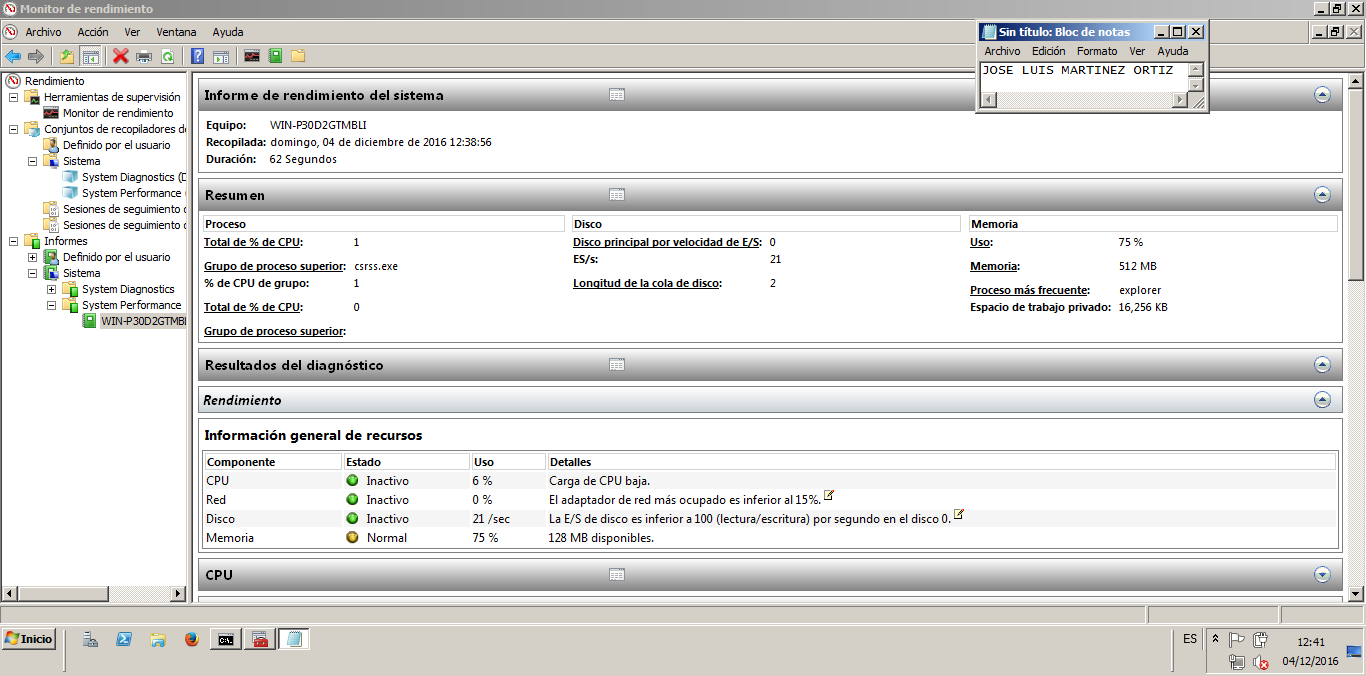
\includegraphics[scale=0.4]{./imagenes/P3_4_1.png} 
\caption{Informe del monitor de rendimiento - resumen} \label{fig:P3_4_1}
\end{figure}




%------------------------------------------------

\bibliography{citas} %archivo citas.bib que contiene las entradas 
\bibliographystyle{plain} % hay varias formas de citar

\end{document}



